\documentclass[12pt]{article}
        \makeatletter
        \def\input@path{{../../}}
        \makeatother
        \usepackage{sbc-template}
        \makeatletter
        \renewcommand{\inst}[1]{}
        \makeatother
        \usepackage{graphicx,url}
        \usepackage[utf8]{inputenc}
        \usepackage[T1]{fontenc}
        \usepackage[brazil]{babel}
        \usepackage{longtable,booktabs,array}
        \usepackage{amsmath,amssymb}
        \providecommand{\tightlist}{%%
          \setlength{\itemsep}{0pt}\setlength{\parskip}{0pt}}
        \sloppy
        \title{Por que Reservoir Computing funciona: memória, não linearidade e capacidade de representação}
        \author{}
        \address{}
        \begin{document}

        \maketitle

        \begin{resumo}
        Este artigo responde a pergunta que ficou aberta depois do primeiro pipeline: por que o desempenho do RC muda tanto quando ajustamos seus hiperparametros? Para responder, conectamos memória, não linearidade e capacidade de representação a resultados computacionais reais do projeto. Começamos por uma leitura teórica do reservatório, mostramos como o \texttt{leak\_rate} controla a escala temporal efetiva, como o \texttt{spectral\_radius} influencia estabilidade e mistura e como o tamanho do reservatório afeta a base de representação. Em seguida, analisamos os resultados de varreduras reais sobre \texttt{n\_reservoir}, \texttt{spectral\_radius} e \texttt{leak\_rate}. O artigo não apenas explica RC em abstrato: ele mostra o que essas ideias produzem, ou destroem, no recorte adotado no Favorita.
        \end{resumo}

        \section{O que o leitor vai aprender}}\label{1-o-que-o-leitor-vai-aprender}

Ao final deste artigo, você será capaz de:

\begin{enumerate}
\def\labelenumi{\arabic{enumi}.}
\tightlist
\item
  explicar memória e não linearidade no RC em termos matemáticos;
\item
  entender por que \texttt{spectral\_radius} e \texttt{leak\_rate} mudam o comportamento do modelo;
\item
  interpretar tabelas de tuning do RC;
\item
  diferenciar capacidade de representação de mera quantidade de unidades;
\item
  decidir o que vale testar antes de partir para QRC.
\end{enumerate}

\section{Memória: o passado precisa continuar presente}}\label{2-memuxf3ria-o-passado-precisa-continuar-presente}

Em RC, a memória não aparece como um vetor de lags explicitamente escrito. Ela aparece no proprio estado do reservatório. Se linearizarmos a dinâmica em torno de uma regiao pequena, obtemos aproximadamente

\[
x_t \approx A x_{t-1} + \alpha W_{in} u_t + \alpha b,
\qquad
A = (1 - \alpha) I + \alpha W_{res}.
\]

Desdobrando a recursao:

\[
x_t \approx \sum_{k=0}^\infty A^k (\alpha W_{in} u_{t-k} + \alpha b).
\]

Essa expressao mostra a intuição correta: o estado atual e uma superposicao ponderada do passado. A velocidade com que o passado "desaparece" depende da matriz efetiva \(A\), logo depende de \texttt{spectral\_radius} e \texttt{leak\_rate}.

\subsection{O papel do leak rate}}\label{21-o-papel-do-leak-rate}

O \texttt{leak\_rate} regula quanto do estado novo substitui o estado antigo. Valores pequenos alongam a memória; valores grandes tornam a resposta mais reativa.

No projeto, o \texttt{leak\_rate} default foi \texttt{0.15}, mas a varredura mostrou que \texttt{0.30} melhora levemente o resultado neste recorte.

\begin{longtable}[]{@{}lllll@{}}
\toprule\noalign{}
leak\_rate & MAE & RMSE & WAPE & sMAPE \\
\midrule\noalign{}
\endhead
\bottomrule\noalign{}
\endlastfoot
0.05 & 388.180 & 491.504 & 0.1793 & 0.1982 \\
0.1 & 357.675 & 474.461 & 0.1652 & 0.1822 \\
0.15 & 324.294 & 423.417 & 0.1498 & 0.1653 \\
0.3 & 317.767 & 419.947 & 0.1467 & 0.1621 \\
0.5 & 770.680 & 1035.544 & 0.3559 & 0.5702 \\
\end{longtable}

Esse resultado ensina uma licao importante: uma memória mais longa não é automaticamente melhor. Se a série responde fortemente a promoção e sazonalidade semanal, uma resposta um pouco mais rapida pode ajudar.

\subsection{O papel do washout}}\label{22-o-papel-do-washout}

O \texttt{washout} separa o regime transiente inicial da dinâmica útil para treino:

\[
\Phi = [\phi_w, \phi_{w+1}, \dots, \phi_T]^\top.
\]

Sem \texttt{washout}, o readout pode aprender artefatos de inicialização em vez de aprender uma representação estabilizada da série.

\section{Não linearidade: por que a série não cabe em uma regra unica}}\label{3-nuxe3o-linearidade-por-que-a-suxe9rie-nuxe3o-cabe-em-uma-regra-unica}

O reservatório usa a não linearidade \texttt{tanh}:

\[
\widetilde{x}_t = \tanh(W_{res} x_{t-1} + W_{in} u_t + b).
\]

Essa não linearidade e o que permite ao modelo misturar efeitos de calendário, promoção e demanda prévia sem impor uma relação puramente aditiva ou puramente linear.

Em previsão de demanda, isso importa porque:

\begin{itemize}
\tightlist
\item
  a mesma promoção pode gerar efeitos diferentes em dias diferentes;
\item
  o mesmo dia da semana pode ter resposta diferente dependendo do histórico imediato;
\item
  a relação entre passado e presente não precisa ser monotona nem linear.
\end{itemize}

\section{Capacidade de representação: tamanho importa, mas não sozinho}}\label{4-capacidade-de-representauxe7uxe3o-tamanho-importa-mas-nuxe3o-sozinho}

Um erro comum de iniciantes e supor que "mais unidades" sempre significa "mais desempenho". A varredura de \texttt{n\_reservoir} no projeto mostra o contrario.

\begin{longtable}[]{@{}lllll@{}}
\toprule\noalign{}
n\_reservoir & MAE & RMSE & WAPE & sMAPE \\
\midrule\noalign{}
\endhead
\bottomrule\noalign{}
\endlastfoot
40 & 1278.623 & 1721.270 & 0.5904 & 0.4393 \\
80 & 324.294 & 423.417 & 0.1498 & 0.1653 \\
120 & 394.030 & 464.884 & 0.1820 & 0.2026 \\
160 & 430.945 & 565.166 & 0.1990 & 0.2359 \\
\end{longtable}

A configuração \texttt{n\_reservoir\ =\ 80} foi a melhor entre as testadas. Quando o reservatório ficou pequeno demais (\texttt{40}), o erro explodiu. Mas aumentar para \texttt{120} e \texttt{160} também piorou.

Esse comportamento sugere que capacidade útil e compatibilidade com o problema importam mais do que simplesmente aumentar a dimensionalidade.

\section{Estabilidade e mistura: o papel do spectral radius}}\label{5-estabilidade-e-mistura-o-papel-do-spectral-radius}

O \texttt{spectral\_radius} reescala a matriz recorrente para controlar o quanto a dinâmica interna amplifica ou dissipa o estado.

\begin{longtable}[]{@{}lllll@{}}
\toprule\noalign{}
spectral\_radius & MAE & RMSE & WAPE & sMAPE \\
\midrule\noalign{}
\endhead
\bottomrule\noalign{}
\endlastfoot
0.2 & 275.280 & 347.305 & 0.1271 & 0.1420 \\
0.4 & 340.569 & 454.497 & 0.1573 & 0.1764 \\
0.6 & 324.294 & 423.417 & 0.1498 & 0.1653 \\
0.8 & 871.792 & 1188.448 & 0.4026 & 0.6992 \\
1.0 & 500.267 & 632.914 & 0.2310 & 0.2519 \\
\end{longtable}

A varredura mostra três regimes didaticamente importantes:

\begin{enumerate}
\def\labelenumi{\arabic{enumi}.}
\tightlist
\item
  \texttt{0.2} produziu o melhor conjunto de métricas entre os valores testados;
\item
  \texttt{0.6} ficou em uma faixa intermediária e foi o default do primeiro pipeline;
\item
  \texttt{0.8} e \texttt{1.0} degradaram muito a estabilidade, com explosao de erro.
\end{enumerate}

Em outras palavras, este recorte prefere um reservatório mais contido do que o default inicial sugeria.

\section{Como ler os hiperparametros do RC no código}}\label{6-como-ler-os-hiperparametros-do-rc-no-cuxf3digo}

O ponto de entrada do tuning esta em \texttt{RCConfig}:

\begin{verbatim}
@dataclass(frozen=True)
class RCConfig:
    n_reservoir: int = 80
    spectral_radius: float = 0.6
    leak_rate: float = 0.15
    input_scale: float = 0.8
    bias_scale: float = 0.1
    washout: int = 14
    ridge_alpha: float = 1e-3
    seed: int = 7
\end{verbatim}

Um modo pratico de estudar o modelo e variar apenas um hiperparametro por vez, mantendo os demais fixos. Foi exatamente isso que os artefatos deste artigo fizeram.

\section{O que o resultado atual do RC sugere}}\label{7-o-que-o-resultado-atual-do-rc-sugere}

\pandocbounded{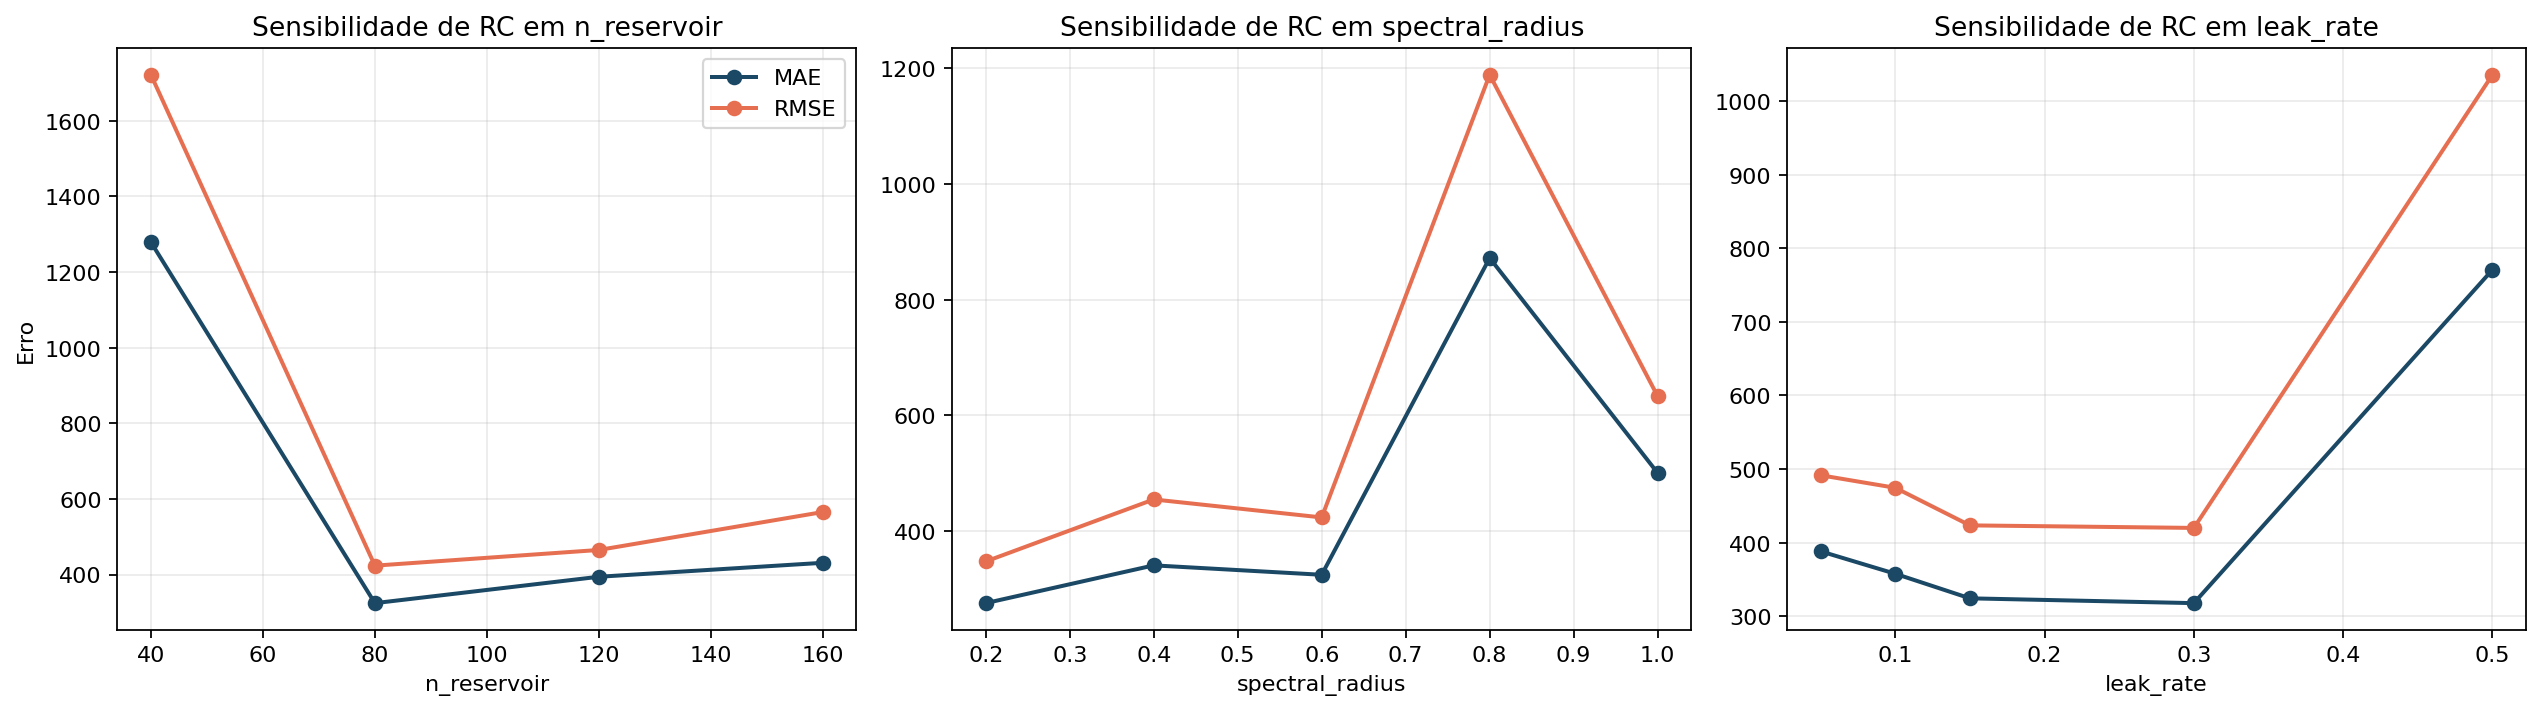
\includegraphics[keepaspectratio,alt={Resumo visual das varreduras de hiperparametros do RC no recorte adotado no Favorita.}]{computational_results_20260402_222902/rc_sensitivity_summary.png}}

O resumo visual permite uma leitura didática direta:

\begin{itemize}
\tightlist
\item
  o modelo e sensivel ao \texttt{spectral\_radius};
\item
  o \texttt{leak\_rate} possui um ponto intermediário útil;
\item
  o tamanho do reservatório tem um regime otimo local, e não monotonia.
\end{itemize}

Isso confirma uma licao central para a série: o RC não deve ser avaliado apenas por uma configuração arbitraria. Seu desempenho depende de como ajustamos memória, mistura e capacidade.

\section{O que RC faz bem e o que ainda não faz bem aqui}}\label{8-o-que-rc-faz-bem-e-o-que-ainda-nuxe3o-faz-bem-aqui}

\subsection{O que RC faz bem}}\label{81-o-que-rc-faz-bem}

\begin{itemize}
\tightlist
\item
  constroi uma representação temporal dinâmica de baixo custo de treinamento;
\item
  absorve sinais de promoção e calendário sem uma engenharia tabular extensa;
\item
  oferece uma ponte conceitual excelente para o QRC.
\end{itemize}

\subsection{O que RC ainda não faz bem aqui}}\label{82-o-que-rc-ainda-nuxe3o-faz-bem-aqui}

\begin{itemize}
\tightlist
\item
  ainda não supera os melhores modelos clássicos neste recorte;
\item
  ainda depende de tuning cuidadoso para evitar instabilidade ou sub-representação;
\item
  ainda não incorpora a riqueza completa do dataset Favorita.
\end{itemize}

\section{Passo-a-passo para reproduzir o estudo de sensibilidade}}\label{9-passo-a-passo-para-reproduzir-o-estudo-de-sensibilidade}

Um leitor que queira repetir este artigo pode seguir esta sequência:

\begin{enumerate}
\def\labelenumi{\arabic{enumi}.}
\tightlist
\item
  executar \texttt{python\ code/rc/run.py} para fixar a configuração base;
\item
  alterar \texttt{RCConfig} em \texttt{code/rc/model.py} ou criar instancias novas em um script de experimento;
\item
  rerodar a previsão para cada combinacao;
\item
  comparar \texttt{MAE}, \texttt{RMSE}, \texttt{WAPE} e \texttt{sMAPE};
\item
  guardar o resultado em CSV e imagem, como foi feito em \texttt{computational\_results\_20260402\_222902/}.
\end{enumerate}

Esse processo prepara o leitor para a fase seguinte da série, em que a comparação deixa de ser apenas "baseline versus RC" e vira um benchmark mais amplo.

\section{Conclusão}}\label{10-conclusuxe3o}

Este artigo mostrou que o RC funciona porque oferece memória distribuída e não linearidade controlada, mas que essa vantagem depende de como configuramos o sistema dinamico. O proprio comportamento das varreduras do projeto ensina essa licao melhor do que qualquer definicao abstrata: parametros inadequados destroem o desempenho, enquanto escolhas razoaveis tornam o reservatório competitivo o suficiente para merecer comparação seria.

\section{Entregaveis associados no repositorio}}\label{entregaveis-associados-no-repositorio}

\begin{itemize}
\tightlist
\item
  implementação do RC: \texttt{code/rc/model.py}
\item
  artefatos de sensibilidade: \texttt{computational\_results\_20260402\_222902/}
\item
  arquivos principais: \texttt{rc\_sweep\_n\_reservoir.csv}, \texttt{rc\_sweep\_spectral\_radius.csv}, \texttt{rc\_sweep\_leak\_rate.csv}, \texttt{rc\_sensitivity\_summary.png}
\end{itemize}

\section{Referencias}}\label{referencias}

\begin{itemize}
\tightlist
\item
  Jaeger, H. The "echo state" approach to analysing and training recurrent neural networks.
\item
  Lukosevicius, M. A practical guide to applying echo state networks.
\item
  Verstraeten, D. et al. Memory versus non-linearity in reservoirs.
\end{itemize}

        \end{document}
